\documentclass[conference]{IEEEtran}
\usepackage{blindtext, graphicx}
\usepackage{color}

\newcommand\todoEB[1]{\textcolor{red}{EB: #1}}

% correct bad hyphenation here
\hyphenation{op-tical net-works semi-conduc-tor}

\begin{document}
\title{Software and Networking infrastructure \\for collaborative IoT Robotics}

\author{
\IEEEauthorblockN{Loic Dauphin}
\IEEEauthorblockA{
Inria, Universit\'e Paris-Saclay\\
loic.dauphin@inria.fr
}
\and
\IEEEauthorblockN{Emmanuel Baccelli}
\IEEEauthorblockA{
Inria, Universit\'e Paris-Saclay\\
emmanuel.baccelli@inria.fr
}
\and
\IEEEauthorblockN{Cedric Adjih}
\IEEEauthorblockA{
Inria, Universit\'e Paris-Saclay\\
cedric.adjih@inria.fr
}
}

\maketitle

\begin{abstract}
To Do.
\end{abstract}

\begin{IEEEkeywords}
IEEEtran, journal, \LaTeX, paper, template.
\end{IEEEkeywords}

\IEEEpeerreviewmaketitle

\section{Robotics/IoT collaboration}

Robots will need to collaborate to fulfill tasks that they cannot do alone at some point.
To collaborate, they need to communicate to each other their "skills" (what they can or cannot do, example : "I can move on an plane floor, but not stairs").
Once all the skills have been collected, compared with a mission statement, a mission plan can be generated.
Once the plan is generated, the controllers can execute this plan via standard communication interfaces.

In the case of robot modularity, where every robot parts can be considered as a standalone system collaborating with others to make a whole robot, this kind of system would enable hardware constructor to focus on the hardware itself.
With a proper description of the hardware skills, a robot could use a new module with no need to modify the robot's software.
This would be even more useful if robots are able to remove/add/replace parts autonomousely.

In the case of a task that is too hard for one robot, the robot could autonomously ask the help of other robots or external sensors to reach it's goals.

The computing power needed for this kind of system is likely to be too high for being embedded, considering the complexity of missions the robots will be needed to accomplish.
There is a need to distribute the computing tasks, or (at least partly) execute it in the cloud, taking advantage of the omnipresence of wireless networking.

\section{Formalization of the problem}

This collaboration problem, as any robotic application, has 3 kind of components : 

\subsection{Environment}

The environment is what a robot can sense or modify, including physical body of the robot.
Basically, the environment can be defined by it's state at time T, which can (and should, in the case of a robot's mission) change over time.

Most of the time, not to say always, the environment will not be entirely known by the robotic application.
A lot of research have been done for environment discovery.
But in the case of an urbanized environement filled with connected sensors (smart homes, factories, ...), robots can take advantage of external sensors, or even partial "a priori" description of the environment (a building's blueprints).

\subsection{Tasks}

The tasks are the way the robots will act on/modify the environment.
A task can be considered as a transition between 2 environment states.
Example : dirty room $\rightarrow$ clean room.

There is 2 types of tasks when a robot is asked to do something : 
 - The high level task the user need to be done, let's call it a "mission".
 - The lower level tasks a robot is able to do, called "actions"

The aim is to find an action sequence (a plan) that will be able to fulfill the mission.

\begin{figure}
  \centering
  \caption{\label{env_graph}Environment states graph}
  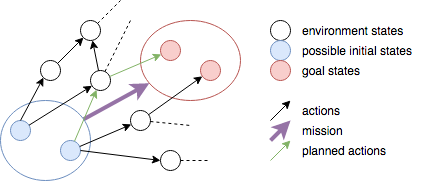
\includegraphics[scale=0.40]{img/env_graph}
\end{figure}

\subsection{Actors (Robots/IoT devices)}

Robots and IoT devices are the executors from which the environment is sensed or modified.

As described previously, the robots are able to do some actions, and will need to execute them in a particular sequence to accomplish a mission.
Since the environment is not completely known, the plan may need to be modified over time.
So, the system making the plan will need a feedback loop to modify it when needed (sense-plan-act ?)

\section{Software architecture}

\begin{figure}
  \centering
  \caption{\label{3layers}Robot collaboration software architecture}
  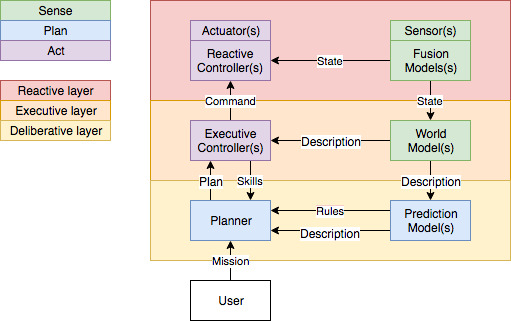
\includegraphics[scale=0.40]{img/3layers}
\end{figure}

The global architecture is a Sense-Plan-Act, but this architecture is not very modular and cannot easily be distributed across several robots.
Also, Sense-Plan-Act is not well suited for the low level control of a robot (especially if the robot is limited in computing power), where Sense-Act is preferred.

The base architecture can be adapted to a 3 layers architecture (Reactive, Executive, Deliberative).
The deliberative layer keebs a Sense-Plan-Act pattern, while the reactive layer will keep the simple and distributed low level control of the robot.

The reactive layer only understand low level, short-termed single commands, while the deliberative layer outputs a plan, consisting of a more or less complex sequence of actions.
The executive layer is here as an adaptation layer between the 2 formers.
It should also be able to express the actions that the planner will be able to use to solve a problem.

\section{Discovery}

To collaborate, robots will need the help of the network to discover each other.
We need to discover the robots endpoints (named/addressed data streams) and the type of data exchanged.

The problem solver / planner part will also need to "understand" what kind of actions the robots can do.
The "skills" can be described with a specific language (PDDL, STRIPS, and co), and served by the robots to be downloaded by the planning part.

There is three steps of the discovery : 
First, after the mission is received, the planning system need to discover which actors (robots/IoT devices) can be used.
Then, it need to dicover the skills of each actors.
And finally, and continuously, the environment need to be discovered through prior knoledge, or sensing.

\section{Planning}

The planning problem can be splitted in 2 parts (PDDL, STRIPS,...) : 
The domain description, which describe the possible states of the manipulated entities (the environement) and the possible actions (of the robots, in our case).
The problem description, which basically describes the initial state, and the goal state.

In the case of robotics, the initial state is not really known, so that the problem description is meant to change over time, and be splitted in 2 : 

The goal state, which does not changes unless the user decide otherwize.
This is the mission of the robot as described previously.

The "initial state", or the current environment state, which will be updated with discovery and envirnment sensing.
Basically, the planning algorithm will be ran periodically (or on input event) with a different initial state description.

\section{Control}

There is 2 types of controllers : 
Reactive controllers, that takes short-termed simple commands, sensors states, and outputs lower leve commands to actuators (or lower level reactive controllers).
Executive controllers, that takes mission plan, environment description, and sends proper commands to one or several reactive controllers.

\section{Recurcivity}

Considering modularity and different level of description of the environment and tasks, planners can be considered as controllers for higher level planners.
Indeed, if during the global mission plan, an action is to "grab object X", this action can be considered as a mission for a lower level planner, that will schedule each action of the robotic arm to fulfill the mission.

\section{bottom-up domain description}

If robots parts can do simple tasks, the parts linked together can do more complex actions that cannot be described in any domain description of the pieces.
There will be a need to automatically compute new possible tasks that can be done by the set of modules, and make it available to the planner.

\section{Communication}

\subsection{Pub/Sub}

This communication pattern is used when we need the data to be sent to the consumer as fast as possible after it has bee produced.
For example, the data of a sensor that is used in a (realtime) control system.
Also, the commands of an controller that is sent to an actuator (real or virtual).

\subsection{Req/Res}

This communication pattern is used when the consumer need a big chunck of data, or data that is not updated often, or when requesting a computation task.
This can be used for example to serve the skills descriptions, where a planned will request only when the robot is discovered.
This can also be used to run some heavy computation on a server if the client is not powerful enough.


\begin{thebibliography}{1}

\bibitem{IEEEhowto:kopka}
H.~Kopka and P.~W. Daly, \emph{A Guide to \LaTeX}, 3rd~ed.\hskip 1em plus
  0.5em minus 0.4em\relax Harlow, England: Addison-Wesley, 1999.

\end{thebibliography}

\end{document}
